
\documentclass[12pt,journal,compsoc]{IEEEtran}
\usepackage{array}
\usepackage{bytefield}
\usepackage{graphicx}
\usepackage{listings}
\usepackage{slashbox}
\usepackage{tikz}
\lstset{
frame=tb,
language=C,
aboveskip=3mm,
belowskip=3mm,
showstringspaces=false,
columns=flexible,
basicstyle={\small\ttfamily},
numbers=none,
breaklines=true,
breakatwhitespace=true,
tabsize=3
}
\hyphenation{op-tical net-works semi-conduc-tor}
\newcounter{mcount}
\setcounter{mcount}{0}
\begin{document}
\title{Chat System}
\author{David Gong, Stephen Hamilton}% <-this % stops a space
\date{Sunday, September 21, 2014}
\IEEEtitleabstractindextext{%
\begin{abstract}
Our goal is to develop a distributed chat server client system that is fault tolerant. 
\end{abstract}
}
\maketitle
\section{Introduction}
\IEEEPARstart{T}{his} system will be composed of a client and a server.  Servers will communicate through spread and utilize multicast with agreed ordering.  
\section{Design}
\subsection{Assumptions}
Below are our assumptions.
\begin{itemize}
\item A user is uniquely identified by their screen name.
\item 
\end{itemize}
\subsection{Chat Message Packet}
\begin{lstlisting}
// Structure of chat packet.
int type;//Type of packet 0 for message, 1 for like
int sequence;//Global ordering of message
char name[25]; //Text name of user
char group[25]; //Text name of chat room
char text[80]; //Text of chat message
int like_sequence; //Integer of sequence number of message liked
\end{lstlisting}
The message packet is utilized for both chat messages and likes created by a user.  The message packet will be saved to disk when received from spread, and the sequence number will be assigned upon receiving it from spread (it is null initially).

\subsection{Server State Machine}
\begin{center}
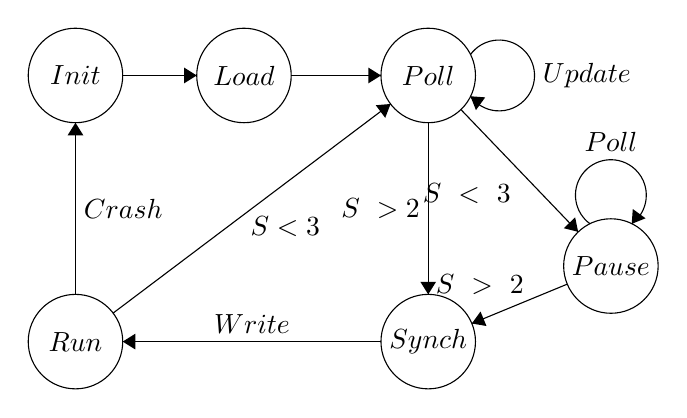
\begin{tikzpicture}[scale=0.2]
\tikzstyle{every node}+=[inner sep=0pt]
\draw [black] (3.3,-3.2) circle (3);
\draw (3.3,-3.2) node {$Init$};
\draw [black] (14,-3.2) circle (3);
\draw (14,-3.2) node {$Load$};
\draw [black] (25.7,-3.2) circle (3);
\draw (25.7,-3.2) node {$Poll$};
\draw [black] (25.7,-20.1) circle (3);
\draw (25.7,-20.1) node {$Synch$};
\draw [black] (3.3,-20.1) circle (3);
\draw (3.3,-20.1) node {$Run$};
\draw [black] (37.3,-15.3) circle (3);
\draw (37.3,-15.3) node {$Pause$};
\draw [black] (27.78,-5.37) -- (35.22,-13.13);
\fill [black] (35.22,-13.13) -- (35.03,-12.21) -- (34.31,-12.9);
\draw (30.97,-10.72) node [left] {$S\mbox{ }<\mbox{ }3$};
\draw [black] (25.7,-6.2) -- (25.7,-17.1);
\fill [black] (25.7,-17.1) -- (26.2,-16.3) -- (25.2,-16.3);
\draw (25.2,-11.65) node [left] {$S\mbox{ }>2$};
\draw [black] (6.3,-3.2) -- (11,-3.2);
\fill [black] (11,-3.2) -- (10.2,-2.7) -- (10.2,-3.7);
\draw [black] (17,-3.2) -- (22.7,-3.2);
\fill [black] (22.7,-3.2) -- (21.9,-2.7) -- (21.9,-3.7);
\draw [black] (22.7,-20.1) -- (6.3,-20.1);
\fill [black] (6.3,-20.1) -- (7.1,-20.6) -- (7.1,-19.6);
\draw (14.5,-19.6) node [above] {$Write$};
\draw [black] (3.3,-17.1) -- (3.3,-6.2);
\fill [black] (3.3,-6.2) -- (2.8,-7) -- (3.8,-7);
\draw (3.8,-11.65) node [right] {$Crash$};
\draw [black] (34.53,-16.45) -- (28.47,-18.95);
\fill [black] (28.47,-18.95) -- (29.4,-19.11) -- (29.02,-18.19);
\draw (28.97,-17.16) node [above] {$S\mbox{ }>\mbox{ }2$};
\draw [black] (35.977,-12.62) arc (234:-54:2.25);
\draw (37.3,-8.05) node [above] {$Poll$};
\fill [black] (38.62,-12.62) -- (39.5,-12.27) -- (38.69,-11.68);
\draw [black] (5.69,-18.29) -- (23.31,-5.01);
\fill [black] (23.31,-5.01) -- (22.37,-5.09) -- (22.97,-5.89);
\draw (16.62,-12.15) node [below] {$S<3$};
\draw [black] (28.38,-1.877) arc (144:-144:2.25);
\draw (32.95,-3.2) node [right] {$Update\mbox{ }$};
\fill [black] (28.38,-4.52) -- (28.73,-5.4) -- (29.32,-4.59);
\end{tikzpicture}
\end{center}

\subsection{Correctness}
Servers will utilize Spread so that each message delivered by spread will be sequenced to ensure all servers maintain an agreed sequence over all messages.  When a server receives a message from spread, it will append the message struct to the server logfile.  This will only occur when in the run state.  If there are not enough servers for a majority, the servers will tell the client that the system is down, and recommend they connect to another server.  Once the server is in the majority partition, they will send the latest agreed sequence number to the first available server to receive updates to the current sequence.  Once they are synchronized, it will run like the other servers.
\\
Upon a loss of a server, if the total number falls below 3, servers will update each other to the latest message, but no longer accept chat messages from users.  Once the number is 3 or more, the servers will send their latest agreed number, and the highest one will update all others lower than that number.\\
\\
When clients send messages, they go to the chat server, and do not appear in the chat room until it is received by the spread daemon and ordered.  When this occurs, the client is updated with their own message in the chat room.
\end{document}
